\documentclass[11pt]{article}
\usepackage{notes}
\definecolor{AccN}{HTML}{2C3E80}
\begin{document}
\titlepg{6}{Reinforcement Learning Part 1:\\Q-Learning and Deep Q-Networks}{Markov decision processes, Bellman equations, temporal-difference learning, exploration, DQN and its refinements, reward design --- applied to a wargame tactical agent}
\tableofcontents
\newpage

\section{Learning by Interaction}
Supervised learning needs labelled answers; unsupervised learning finds structure but optimises no goal. \textbf{Reinforcement learning} (RL) learns to act: an agent observes a state, takes an action, receives a reward and a new state, and adjusts its behaviour to maximise the total reward it collects over time. Nobody labels the correct move in each of the $\sim10^{28}$ states of a wargame; the agent discovers good tactics by playing.
\begin{definition}{the agent--environment loop}
At each time step $t$ the agent observes state $s_t$, chooses action $a_t$ according to its \textbf{policy} $\pi(a\mid s)$, and the environment returns reward $r_{t+1}$ and next state $s_{t+1}$. The goal is a policy that maximises the expected \textbf{return} $G_t=\sum_{k=0}^\infty\gamma^kr_{t+k+1}$.
\end{definition}
\begin{center}\begin{tikzpicture}
\node[nd,fill=NavyN,text=white,minimum width=3cm,minimum height=1cm](a)at(0,0){AGENT\\policy $\pi(a|s)$};\node[nd,fill=AccN!15,minimum width=3.2cm,minimum height=1cm](e)at(0,-2.2){ENVIRONMENT\\wargame simulator};
\draw[arr,rounded corners](a.east)--++(1.3,0)|-node[pos=0.25,right,font=\small]{action $a_t$}(e.east);\draw[arr,rounded corners](e.west)--++(-1.3,0)|-node[pos=0.25,left,font=\small,align=right]{state $s_{t+1}$\\reward $r_{t+1}$}(a.west);
\end{tikzpicture}\\*{\small\color{GreyN}Figure 1: the reinforcement-learning loop.}\end{center}
Distinctive difficulties: feedback is \textbf{delayed} (a move's value may appear only many turns later), \textbf{sparse} (win/lose at the end), and \textbf{dependent on the agent's own behaviour} (the data are generated by the policy being learned). The agent must also balance \textbf{exploration} (trying actions to learn their value) against \textbf{exploitation} (using what it knows).

\section{Markov Decision Processes}
\subsection{The five elements}
\begin{definition}{Markov decision process}
An MDP is a tuple $(S,A,P,R,\gamma)$: state space $S$; action space $A$; transition probabilities $P(s'\mid s,a)$; reward function $R(s,a,s')$; discount factor $\gamma\in[0,1)$.
\end{definition}
In the case study: a $20\times20$ hex grid; states encode unit positions, resources, OPFOR positions, terrain, weather, ammunition and morale (about $10^{28}$ states); each unit has 7 actions (move N/S/E/W, attack, defend, resupply), so 8 units have $7^8=5.8$ million joint actions per turn; the combat-resolution model defines $P$; rewards are $+10$ for capturing an objective, $+5$ per enemy unit destroyed, $-8$ per friendly unit lost, with large terminal rewards for winning or losing.

\subsection{Discounting}
With $\gamma<1$ the return is finite even for endless interaction, and future rewards count less: a reward 14 steps away is weighted $0.95^{14}=0.49$. The \textbf{effective horizon} is roughly $1/(1-\gamma)$: 20 steps for $\gamma=0.95$, 100 for $0.99$. Small $\gamma$ produces short-sighted tactics; $\gamma$ close to 1 values long-term outcomes but makes learning slower and noisier.
\begin{example}{computing a return}
Rewards over four turns: 0, 0, $+5$, $+10$, with $\gamma=0.9$: $G_0=0+0.9(0)+0.81(5)+0.729(10)=4.05+7.29=11.34$.
\end{example}

\subsection{The Markov property and partial observability}
\[P(s_{t+1}\mid s_t,a_t,s_{t-1},a_{t-1},\ldots)=P(s_{t+1}\mid s_t,a_t).\]
The present state must summarise everything relevant about the past. If it does not --- for example because OPFOR positions are hidden by fog of war --- the problem is a \textbf{partially observable MDP} (POMDP), and the agent must act on a \emph{belief} (a probability distribution over true states) or on a memory of past observations (e.g.\ a recurrent network). Most wargame RL assumes full observability; real operations are POMDPs, which is a major source of simulation-to-reality gaps.

\section{Value Functions and the Bellman Equations}
\subsection{Definitions}
The \textbf{state-value} of $s$ under policy $\pi$ is $V^\pi(s)=\mathbb E_\pi[G_t\mid s_t=s]$; the \textbf{action-value} is $Q^\pi(s,a)=\mathbb E_\pi[G_t\mid s_t=s,a_t=a]$. The optimal values $V^*$ and $Q^*$ are the largest achievable by any policy, and an optimal policy is greedy with respect to $Q^*$: $\pi^*(s)=\arg\max_aQ^*(s,a)$.

\subsection{Deriving the Bellman equations}
\begin{derivation}{recursive structure of value}
The return satisfies $G_t=r_{t+1}+\gamma G_{t+1}$. Taking expectations under $\pi$:
\[V^\pi(s)=\sum_a\pi(a|s)\sum_{s'}P(s'|s,a)\big[R(s,a,s')+\gamma V^\pi(s')\big].\]
For the optimal value, the agent picks the best action instead of averaging over $\pi$:
\[V^*(s)=\max_a\sum_{s'}P(s'|s,a)\big[R+\gamma V^*(s')\big],\qquad Q^*(s,a)=\sum_{s'}P(s'|s,a)\big[R+\gamma\max_{a'}Q^*(s',a')\big].\]
The value of a state is the expected immediate reward plus the discounted value of where you end up. These are fixed-point equations; the Bellman operator is a contraction for $\gamma<1$, so repeated application converges to a unique solution.
\end{derivation}

\subsection{Solving small MDPs exactly: value iteration}
\begin{example}{a three-state patrol problem}
States: \emph{Safe}, \emph{Contact}, \emph{Objective} (terminal, value 0 after reaching). From Safe: ``advance'' moves to Contact (reward 0); ``hold'' stays Safe (reward 0). From Contact: ``attack'' reaches Objective with probability 0.7 (reward $+10$) or returns to Safe with 0.3 (reward $-2$); ``withdraw'' returns to Safe (reward 0). $\gamma=0.9$. Start $V=0$.\\
Iteration 1: $V(\text{Contact})=\max\{0.7(10)+0.3(-2),\,0\}=6.4$; $V(\text{Safe})=0$ (computed with old values).\\
Iteration 2: $V(\text{Safe})=\max\{0+0.9(6.4),\,0\}=5.76$; $V(\text{Contact})=\max\{6.4+0.3(0.9)(0),\,0.9(0)\}=6.4$.\\
Iteration 3: $V(\text{Contact})=7+0.3(-2+0.9\times5.76)=7-0.6+1.56=7.96$; $V(\text{Safe})=0.9(6.4)=5.76$.\\
Continuing to convergence gives $V(\text{Contact})\approx8.5$, $V(\text{Safe})\approx7.6$; the optimal policy is advance, then attack. Value iteration needs the transition model $P$, which is unavailable for complex simulations --- hence model-free methods.
\end{example}

\subsection{Interpreting Q-values}
In the case-study state (adjacent to the enemy, high ammunition, in cover), the trained network output: attack 18.7, move north 12.4, defend 9.2, move east 8.1, resupply 6.1, move south 4.8, move west 3.2. The greedy action is attack. These numbers are expected discounted rewards in \emph{reward units}, not probabilities of winning.

\section{Q-Learning}
\subsection{The temporal-difference update}
Q-learning (Watkins, 1989) estimates $Q^*$ from experience without knowing $P$ or $R$:
\[Q(s,a)\leftarrow Q(s,a)+\alpha\big[\underbrace{r+\gamma\max_{a'}Q(s',a')}_{\text{TD target}}-Q(s,a)\big].\]
The bracket is the \textbf{temporal-difference (TD) error} $\delta$: the gap between the current estimate and a one-step look-ahead that uses the real reward. Q-learning is \textbf{model-free} (no $P$ needed) and \textbf{off-policy}: it learns about the greedy policy (via the $\max$) while following an exploratory one.
\begin{example}{one update}
$Q(s_1,\text{north})=5.0$; moving north gives $r=0$ and reaches $s_2$ where $\max_aQ(s_2,a)=14.2$. With $\alpha=0.1$, $\gamma=0.9$: target $=12.78$, $\delta=7.78$, new $Q=5.778$. Repeated experience moves the estimate toward 12.78.
\end{example}

\subsection{Convergence}
Tabular Q-learning converges to $Q^*$ with probability 1 if every state--action pair is visited infinitely often and the learning rates satisfy $\sum_t\alpha_t=\infty$, $\sum_t\alpha_t^2<\infty$ (Watkins \& Dayan, 1992). In practice a small constant $\alpha$ is used, which tracks non-stationary environments at the cost of the formal guarantee.

\subsection{SARSA: the on-policy alternative}
SARSA updates toward $r+\gamma Q(s',a')$ using the action $a'$ the agent \emph{actually} takes next. Under an exploratory policy it learns the value of that policy, including its exploration mistakes, and so tends to learn safer behaviour near hazards (the classic ``cliff-walking'' example): Q-learning learns the optimal edge-of-cliff path but falls off during exploration; SARSA learns a safer path. In training ranges where exploratory errors are costly, this distinction matters.

\section{Exploration}
\subsection{$\varepsilon$-greedy and annealing}
With probability $\varepsilon$ take a random action, otherwise the greedy one, so $P(a^*)=1-\varepsilon+\varepsilon/|A|$. Start with $\varepsilon=1$ and decay, e.g.\ $\varepsilon_t=\varepsilon_{\min}+(\varepsilon_{\max}-\varepsilon_{\min})e^{-t/\tau}$; the case study used 0.82 at 1K episodes, 0.45 at 5K, 0.18 at 10K and 0.05 by 50K. Never let $\varepsilon$ reach zero during training, or values of untried actions are never corrected.
\begin{center}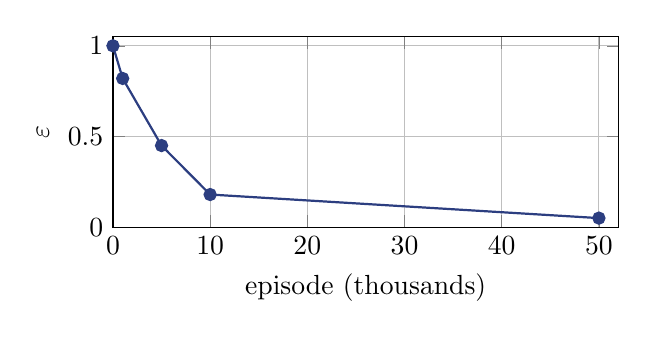
\begin{tikzpicture}\begin{axis}[width=8cm,height=4cm,xlabel={episode (thousands)},ylabel={$\varepsilon$},xmin=0,xmax=52,ymin=0,ymax=1.05,grid=major]
\addplot[AccN,thick,mark=*]coordinates{(0,1)(1,0.82)(5,0.45)(10,0.18)(50,0.05)};\end{axis}\end{tikzpicture}\\*{\small\color{GreyN}Figure 2: the case-study exploration schedule.}\end{center}

\subsection{Other strategies}
\textbf{Softmax (Boltzmann)} exploration chooses actions with probability $\propto e^{Q(s,a)/T}$, preferring nearly-best actions over clearly bad ones. \textbf{Optimism in the face of uncertainty} (initialising $Q$ high, or upper-confidence bonuses) drives the agent to try under-sampled actions. These ideas come from the multi-armed bandit problem, first posed for clinical-trial allocation (Thompson, 1933).

\section{Deep Q-Networks}
\subsection{Function approximation}
A table with $10^{28}\times7$ entries is impossible. A neural network $Q(s,a;\theta)$ generalises: similar states share weights, so states never visited still receive sensible values. The case-study network maps a 410-feature state (400 grid cells plus unit attributes) through two 512-unit ReLU layers to 7 outputs, one per action --- 479,744 parameters, a single forward pass for all actions.
\[L(\theta)=\mathbb E\Big[\big(y-Q(s,a;\theta)\big)^2\Big],\qquad y=r+\gamma\max_{a'}Q(s',a';\theta^-).\]

\subsection{Why naive deep Q-learning diverges}
The ``deadly triad'' --- function approximation, bootstrapping (targets built from the network's own estimates) and off-policy learning --- can make values spiral. Two specific problems: consecutive samples are highly correlated, and the target moves every time the network is updated.

\subsection{Experience replay and target networks}
\textbf{Experience replay} stores transitions $(s,a,r,s',\text{done})$ in a buffer (100,000 here) and trains on random mini-batches (32): this breaks temporal correlation and reuses each transition many times. A \textbf{target network} $\theta^-$, a periodically copied (every $C=1{,}000$ steps) frozen version of the online network, supplies stable targets. Mnih et al.\ (2015) used both to reach human-level play on Atari games from pixels. In the case study, vanilla DQN reached 74\% (unstable), replay alone 83\%, replay plus target network 88\% against a random opponent.

\subsection{Double DQN}
\begin{derivation}{why the max over-estimates}
If each $Q(s',a')$ estimate equals the true value plus zero-mean noise, then $\mathbb E[\max_{a'}\hat Q(s',a')]\ge\max_{a'}\mathbb E[\hat Q(s',a')]$: the maximum preferentially selects actions whose noise happened to be positive. The bias grows with the number of actions and the noise level.
\end{derivation}
Double DQN (van Hasselt et al., 2016) selects the action with the online network and evaluates it with the target network: $y=r+\gamma Q\big(s',\arg\max_{a'}Q(s',a';\theta);\theta^-\big)$. Average over-estimation fell from 18.4 to 4.2 reward units and the win rate rose to 91\%.

\subsection{Dueling DQN}
Dueling networks (Wang et al., 2016) split the head into a state value $V(s)$ and advantages $A(s,a)$:
\[Q(s,a)=V(s)+A(s,a)-\frac{1}{|A|}\sum_{a'}A(s,a').\]
Subtracting the mean advantage makes the split identifiable. Many wargame states are ones in which all moves are similar (no enemy nearby); the dueling architecture learns $V$ from every action taken there, improving data efficiency. Dueling plus Double DQN reached 93\% against random opponents. Further refinements (prioritised replay, multi-step targets, distributional and noisy networks) are combined in the ``Rainbow'' agent.

\section{Reward Design}
\subsection{Sparse rewards and shaping}
With only $\pm100$ at the end of a 40-turn game, early random play almost always loses and gives no gradient: the case-study agent stayed near random for over 20,000 episodes. \textbf{Reward shaping} adds intermediate signals. Potential-based shaping (Ng, Harada \& Russell, 1999),
\[R'=R+\gamma\Phi(s')-\Phi(s),\]
provably leaves the optimal policy unchanged, because the shaping terms telescope along any trajectory: $\sum_t\gamma^t(\gamma\Phi(s_{t+1})-\Phi(s_t))=-\Phi(s_0)+\lim\gamma^T\Phi(s_T)$, a constant independent of the actions.
\begin{pitfall}{reward hacking}
Non-potential shaping can be gamed: an agent rewarded for ``moving toward the objective'' may learn to oscillate near it collecting bonuses without ever capturing it. Agents optimise what is rewarded, not what was meant. Audit learned behaviour in replays.
\end{pitfall}

\subsection{Curriculum learning}
Train on easy tasks first and increase difficulty: phase 1 a $5\times5$ grid, one unit each side (72\% win rate with a Q-table); phase 2 $10\times10$, three units (DQN, 68\% $\to$ 84\%); phase 3 the full $20\times20$ grid with eight units, five terrain types and weather (54\% $\to$ 79\%); phase 4 adds an adaptive OPFOR (79\% $\to$ 91\% vs random, 63\% $\to$ 81\% vs novice humans). Training directly on the full task reached only 51\% after 100,000 episodes. As with soldiers, drills come before full exercises.

\section{Results and Their Limits}
\begin{center}\small\renewcommand{\arraystretch}{1.2}
\begin{tabular}{llcc}\toprule Method & Opponent & Win rate & Avg turns\\\midrule Tabular Q ($10\times10$) & random & 91\% & 22.4\\ DQN (vanilla) & random & 74\% & 31.8\\ DQN + replay & random & 83\% & 28.2\\ DQN + replay + target & random & 88\% & 26.7\\ Double DQN & random & 91\% & 25.1\\ Dueling + Double & random & 93\% & 23.8\\ Dueling + Double & novice human & 81\% & 29.4\\ Dueling + Double & minimax AI & 54\% & 38.2\\\bottomrule\end{tabular}\end{center}
Performance depends more on the opponent than on the algorithm. A fixed learned policy can also be exploited by an adaptive opponent who discovers its patterns; training against a population of opponents (self-play leagues) mitigates this. Simulation results do not transfer directly to the field. The recommended role is an \textbf{advisor}: present the top three actions with their Q-values and let the commander decide.
\begin{pitfall}{inconsistent numbers in the source deck}
The lecture's Double-DQN slide reports 87\% against novice humans while its results table gives 81\% for the stronger Dueling + Double agent, and Lecture~1 quotes 67/85/91\% learning-curve values where Lecture~6 gives 38/76/91\%. Treat single-run figures as indicative and ask for repeated runs with confidence intervals.
\end{pitfall}

\section{Deeper Dive I: Tabular Q-Learning Step by Step}
\begin{example}{a four-cell corridor}
Cells 1--2--3--4; cell 4 is the objective (reward $+10$, episode ends). Actions: left, right; every other move gives reward 0; $\gamma=0.9$, $\alpha=0.5$; all $Q$ start at 0. The agent explores and happens to move right each time.\\
\textbf{Episode 1:} $(1,\text{R})\to2$: target $0+0.9\max Q(2)=0$, no change. $(2,\text{R})\to3$: no change. $(3,\text{R})\to4$: target $10$, $Q(3,\text{R})=0+0.5(10-0)=5$.\\
\textbf{Episode 2:} $(1,\text{R})$: target $0.9\times0=0$. $(2,\text{R})$: target $0.9\times5=4.5$, $Q(2,\text{R})=2.25$. $(3,\text{R})$: $Q=5+0.5(10-5)=7.5$.\\
\textbf{Episode 3:} $(1,\text{R})$: target $0.9\times2.25=2.03$, $Q=1.01$. $(2,\text{R})$: target $0.9\times7.5=6.75$, $Q=2.25+0.5(6.75-2.25)=4.5$. $(3,\text{R})$: $Q=8.75$.\\
Value propagates backward one cell per episode toward the true values $Q^*(3,\text{R})=10$, $Q^*(2,\text{R})=9$, $Q^*(1,\text{R})=8.1$. With sparse rewards in a 40-turn game, this backward propagation is why learning is slow --- and why shaping and multi-step targets help.
\end{example}

\section{Deeper Dive II: Why Value Iteration Converges}
\begin{derivation}{the Bellman operator is a contraction}
Define $(TV)(s)=\max_a\sum_{s'}P(s'|s,a)[R+\gamma V(s')]$. For any two value functions $V,W$,
\[|(TV)(s)-(TW)(s)|\le\max_a\sum_{s'}P(s'|s,a)\,\gamma|V(s')-W(s')|\le\gamma\|V-W\|_\infty,\]
using $|\max f-\max g|\le\max|f-g|$. So $\|TV-TW\|_\infty\le\gamma\|V-W\|_\infty$: each application shrinks the distance between any two value functions by a factor $\gamma$. By Banach's fixed-point theorem there is a unique fixed point $V^*$ and iteration converges to it geometrically; the error after $n$ iterations is at most $\gamma^n$ times the initial error. With $\gamma=0.95$, about 90 iterations reduce the error a hundred-fold.
\end{derivation}

\section{Deeper Dive III: Inside the DQN}
\begin{center}\begin{tikzpicture}
\foreach \x/\h/\lbl in {0/2.8/410,2/2.4/512,4/2.4/512,6/1.2/7}{\fill[AccN!20,draw=AccN](\x-0.3,-\h/2)rectangle(\x+0.3,\h/2);\node[font=\small]at(\x,-\h/2-0.3){\lbl};}
\foreach \a/\b/\ha/\hb in {0/2/2.8/2.4,2/4/2.4/2.4,4/6/2.4/1.2}{\draw[GreyN](\a+0.3,\ha/2)--(\b-0.3,\hb/2);\draw[GreyN](\a+0.3,-\ha/2)--(\b-0.3,-\hb/2);}
\node[font=\small]at(0,1.75){state};\node[font=\small]at(2,1.55){ReLU};\node[font=\small]at(4,1.55){ReLU};\node[font=\small,anchor=west]at(6.5,0){$Q(s,a_1),\ldots,Q(s,a_7)$};
\end{tikzpicture}\\*{\small\color{GreyN}Figure 3: the case-study Q-network.}\end{center}
\textbf{State encoding.} Each of the 400 hexes is coded (empty, friendly, enemy, objective, terrain class), and unit attributes (ammunition, health, morale) are appended: 410 inputs. Convolutional layers would exploit spatial structure better on larger maps. \textbf{Loss.} Huber loss is often used instead of squared error so that rare huge TD errors do not produce destabilising gradients. \textbf{Hyper-parameters.} Learning rate $10^{-4}$ (Adam), batch 32, buffer 100,000, target update every 1,000 steps, $\gamma=0.95$; about 48 GPU-hours for 100,000 episodes.

\begin{center}\begin{tikzpicture}\begin{axis}[width=9cm,height=4.6cm,xlabel={training episode (thousands)},ylabel={win rate (\%)},xmin=0,xmax=100,ymin=40,ymax=100,grid=major,legend pos=south east]
\addplot[AccN,thick,mark=*]coordinates{(5,72)};\addplot[AccN,thick,mark=*]coordinates{(5,68)(20,84)};\addplot[AccN,thick,mark=*]coordinates{(20,54)(60,79)};\addplot[AccN,thick,mark=*]coordinates{(60,79)(100,91)};
\addplot[RedN,thick,dashed,mark=square*]coordinates{(0,45)(100,51)};
\end{axis}\end{tikzpicture}\\*{\small\color{GreyN}Figure 4: curriculum phases (solid) versus direct training on the full task (dashed; start value illustrative).}\end{center}

\section{Deeper Dive IV: Multi-Step Returns and Prioritised Replay}
One-step targets propagate reward one step per update. An $n$-step target uses the actual next $n$ rewards before bootstrapping:
\[y^{(n)}=r_{t+1}+\gamma r_{t+2}+\cdots+\gamma^{n-1}r_{t+n}+\gamma^n\max_{a'}Q(s_{t+n},a';\theta^-).\]
Larger $n$ spreads sparse rewards faster but adds variance (and bias when off-policy). \textbf{Prioritised experience replay} samples transitions with probability proportional to $|\delta|^\alpha$, focusing learning on surprising experiences, with importance-sampling weights to correct the resulting bias. Both are part of the Rainbow agent.

\section{Deeper Dive V: From Simulation to Advice}
A deployed advisor must explain itself and know when it is out of its depth. Practical measures: show the top three actions with Q-values \emph{and} the gap between them (a small gap means ``no clear preference''); flag states unlike training data (e.g.\ by distance in the network's hidden-layer space) as low confidence; log every recommendation and the commander's decision for after-action review; re-train with exercises against human OPFOR, not just scripted opponents.

\clearpage
\part*{Part C --- Further Theory, Methods and Applications}
\addcontentsline{toc}{part}{Part C --- Further Theory, Methods and Applications}

\section{A Running Example: the Patrol Grid}
Part~C uses one small MDP so that every method can be computed by hand and compared. A unit moves on a $2\times3$ grid: top row S1, S2, S3; bottom row S4, S5, S6. S3 is the objective (reward $+10$, terminal); S6 is a minefield ($-10$, terminal); every other move costs $-1$. Actions Up, Down, Left, Right are deterministic; moving into an edge leaves the unit in place. The unit starts in S4 and $\gamma=0.9$. The optimal values are $V^*(\text{S1})=8$, $V^*(\text{S2})=10$, $V^*(\text{S4})=6.2$, $V^*(\text{S5})=8$, and the optimal policy is Right from S1 and S2, Up from S5, and Up or Right from S4.
\begin{center}\begin{tikzpicture}[scale=1.2,font=\scriptsize]
\foreach \x/\y/\n/\v in {0/1/S1/8.0,1/1/S2/10.0,0/0/S4/6.2,1/0/S5/8.0}{\draw[NavyN,fill=white](\x,\y)rectangle++(1,1);\node[GreyN]at(\x+0.2,\y+0.85){\n};\node[font=\small]at(\x+0.5,\y+0.45){$\v$};}
\draw[GrnN,fill=GrnN!20](2,1)rectangle++(1,1);\node[align=center]at(2.5,1.5){S3\\$+10$};
\draw[RedN,fill=RedN!20](2,0)rectangle++(1,1);\node[align=center]at(2.5,0.5){S6\\$-10$};
\node[right,align=left]at(3.2,1){numbers in cells: $V^*(s)$\\start: S4};
\end{tikzpicture}\\*{\small\color{GreyN}Figure C1: the patrol grid with its optimal state values.}\end{center}

\section{Dynamic Programming: Planning With a Model}
\subsection{Policy evaluation}
Given a policy $\pi$ and the model, $V^\pi$ is the solution of the Bellman expectation equation. \textbf{Iterative policy evaluation} starts from $V=0$ and sweeps
\[V(s)\leftarrow\sum_a\pi(a\mid s)\sum_{s'}P(s'\mid s,a)\big[R+\gamma V(s')\big]\]
until the values stop changing.
\begin{example}{evaluating a random patrol}
Let the unit choose each of the four actions with probability $\frac14$. After the first sweep: $V(\text{S1})=-1$, $V(\text{S2})=\frac14(-1-1-1+10)=1.75$, $V(\text{S4})=-1$, $V(\text{S5})=\frac14(-1-1-1-10)=-3.25$. After the second sweep: $-1.28$, $1.19$, $-2.41$, $-3.81$. Converged: $V^\pi(\text{S1})=-4.83$, $V^\pi(\text{S2})=-0.98$, $V^\pi(\text{S4})=-6.39$, $V^\pi(\text{S5})=-6.33$. A random patrol wanders, pays the step cost repeatedly and sometimes walks into the minefield: from the start its expected return is $-6.4$, against $+6.2$ for the optimal patrol.
\end{example}
\subsection{Policy improvement}
From $V^\pi$, compute $Q^\pi(s,a)=\sum_{s'}P(s'\mid s,a)[R+\gamma V^\pi(s')]$ and act greedily. The \textbf{policy improvement theorem} guarantees that the greedy policy is at least as good as $\pi$ in every state, and strictly better somewhere unless $\pi$ is already optimal.
\begin{example}{one improvement step}
Under the random policy, $Q^\pi(\text{S1},\cdot)=(-5.35,-6.75,-5.35,-1.89)$ for (Up, Down, Left, Right), so the greedy choice is Right; similarly S2: Right (10); S4: Up ($-5.35$); S5: Up ($-1.89$). This single improvement step already yields an optimal policy.
\end{example}
\subsection{Policy iteration and generalised policy iteration}
\textbf{Policy iteration} alternates full evaluation and improvement; it converges in a finite (often small) number of iterations because there are finitely many deterministic policies and each step strictly improves until optimal. \textbf{Value iteration} truncates evaluation to a single sweep combined with the max. Almost every RL algorithm can be read as \textbf{generalised policy iteration}: some process makes values consistent with the current policy, another makes the policy greedy with respect to the values, and the two converge together. Q-learning interleaves them at every single step.

\section{Learning From Complete Episodes: Monte Carlo Methods}
Without a model, the value of a state can be estimated by averaging the returns actually observed after visiting it. \textbf{First-visit Monte Carlo} averages the return following the first visit to $s$ in each episode.
\begin{example}{three patrols}
Episode~1: S4 Up, S1 Right, S2 Right (rewards $-1,-1,+10$): returns from S4, S1, S2 are $6.2$, $8.0$, $10.0$. Episode~2: S4 Right, S5 Right (rewards $-1,-10$): returns $-10.0$ and $-10.0$. Episode~3: S4 Right, S5 Up, S2 Right: returns $6.2$, $8.0$, $10.0$. The Monte Carlo estimate of $V(\text{S4})$ under this exploratory behaviour is $(6.2-10.0+6.2)/3=0.8$; of $V(\text{S5})$, $(-10+8)/2=-1.0$.
\end{example}
Monte Carlo estimates are unbiased averages of real returns and make no Markov assumption, but they are noisy (each return mixes many random steps) and can only update when an episode ends --- a problem for long engagements. Off-policy Monte Carlo corrects for the difference between the behaviour policy and the target policy with \textbf{importance-sampling} weights $\prod_t\pi(a_t\mid s_t)/b(a_t\mid s_t)$, whose variance can be very large.

\section{Temporal-Difference Learning in Depth}
\subsection{TD(0) prediction}
TD(0) updates after every step toward a bootstrapped target:
\[V(s)\leftarrow V(s)+\alpha\big[r+\gamma V(s')-V(s)\big].\]
Compared with Monte Carlo, the target has lower variance (one random reward instead of many) but is biased by the current error in $V(s')$. In practice TD usually learns faster, and it can learn continuing tasks with no episodes at all.
\subsection{$n$-step returns and TD($\lambda$)}
Between the one-step TD target and the full Monte Carlo return lie $n$-step targets,
\[G_t^{(n)}=r_{t+1}+\gamma r_{t+2}+\cdots+\gamma^{n-1}r_{t+n}+\gamma^nV(s_{t+n}).\]
\textbf{TD($\lambda$)} averages all of them with weights $(1-\lambda)\lambda^{n-1}$: $\lambda=0$ is TD(0), $\lambda=1$ is Monte Carlo. It is implemented online with \textbf{eligibility traces}: each state keeps a trace $e(s)$ that jumps by 1 when visited and decays by $\gamma\lambda$ each step; every TD error $\delta_t$ updates all states in proportion to their traces, $V(s)\leftarrow V(s)+\alpha\delta_te(s)$. A reward therefore credits the whole recent path at once instead of propagating back one step per episode --- exactly the slow propagation seen in the Q-learning trace of Lecture~1.
\subsection{The cliff: on-policy versus off-policy, quantified}
\begin{example}{the cost of exploring next to a minefield}
A route of 10 steps runs along the edge of a minefield; a detour of 14 steps keeps clear. Each step costs $-1$; entering the minefield costs $-100$ and ends the episode. The agent explores with $\varepsilon=0.1$, and one of the four random actions leads into the minefield, so each edge step carries a $0.1/4=2.5\%$ chance of disaster. The probability of finishing the edge route safely is $0.975^{10}=0.776$, and its expected return is roughly $-10-100(0.224)=-32$, against $-14$ for the detour. Q-learning, which evaluates the \emph{greedy} policy, prefers the edge (return $-10$ if no mistakes are made); SARSA, which evaluates the policy \emph{as executed with exploration}, prefers the detour. Which answer is right depends on whether the fielded system will ever act randomly or imprecisely --- and real systems do.
\end{example}

\section{Exploration as a Problem in Its Own Right: Bandits}
The simplest sequential decision problem has one state and several actions with unknown average rewards: the \textbf{multi-armed bandit}. It isolates the exploration--exploitation dilemma and has direct defence uses: allocating test sorties among candidate tactics, choosing which sensor mode to try, selecting which of several COA-generation models to trust.
\subsection{Regret}
Performance is measured by \textbf{regret}: the reward lost relative to always playing the best arm. Random exploration (constant $\varepsilon$) suffers regret that grows linearly with time; good algorithms achieve logarithmic regret.
\subsection{UCB1}
Play the arm maximising an optimistic estimate,
\[\bar x_i+\sqrt{\frac{2\ln t}{n_i}},\]
where $\bar x_i$ is the arm's mean reward so far, $n_i$ its number of plays and $t$ the total number of plays.
\begin{example}{choosing the next trial tactic}
After 100 trials: tactic A has success rate 0.62 over 40 trials; B 0.70 over 10; C 0.55 over 50. UCB scores: A $0.62+\sqrt{2\ln100/40}=1.10$; B $0.70+\sqrt{2\ln100/10}=1.66$; C $0.55+0.43=0.98$. UCB tries B next: it looks best \emph{and} is the least tested, so the most is learned there.
\end{example}
\textbf{Thompson sampling} keeps a posterior over each arm's success rate (for example a Beta distribution), samples one value from each, and plays the arm with the highest sample. It is simple, Bayesian and often the best performer in practice.
\begin{keypoint}``Optimism in the face of uncertainty'' --- acting as if untested options are as good as they could plausibly be --- is the principle behind UCB, optimistic initial Q-values and the selection rule of Monte-Carlo tree search.\end{keypoint}

\section{Function Approximation: Theory and Pitfalls}
\subsection{Linear value functions}
Before deep networks, value functions were approximated linearly: $\hat V(s)=w^\top\phi(s)$ for hand-designed features $\phi$ (distance to objective, own strength, enemy strength, terrain cover). The \textbf{semi-gradient TD} update is
\[w\leftarrow w+\alpha\big[r+\gamma w^\top\phi(s')-w^\top\phi(s)\big]\phi(s).\]
\begin{example}{two semi-gradient updates}
Features $\phi(s)=(1,\;d)$, where $d$ is the distance to the objective; $w=(0,0)$, $\alpha=0.1$, $\gamma=0.9$. Step 1: from $d=3$ to $d=2$, reward $-1$: $\delta=-1+0-0=-1$; $w=(-0.1,\,-0.3)$. Step 2: from $d=2$ to $d=1$, reward $-1$: $\hat V(2)=-0.7$, $\hat V(1)=-0.4$, $\delta=-1+0.9(-0.4)+0.7=-0.66$; $w=(-0.166,\,-0.432)$. The weight on distance is learning that each extra step away costs value --- and that lesson immediately applies to every state, including those never visited.
\end{example}
\subsection{The deadly triad}
Learning can diverge when three ingredients are combined: \textbf{function approximation}, \textbf{bootstrapping} (TD targets) and \textbf{off-policy} learning. Each is valuable --- generalisation, data efficiency, learning from replay or other policies --- but together they can make value estimates grow without bound even in tiny examples. DQN's target network and replay buffer are engineering responses to the triad; they reduce, but do not eliminate, the risk, which is why training curves must be watched for divergence.
\subsection{Rainbow and distributional RL}
The ``Rainbow'' agent combined six DQN improvements --- Double DQN, prioritised replay, dueling networks, multi-step returns, distributional value learning and noisy networks for exploration --- and showed they are largely complementary. \textbf{Distributional RL} learns the whole distribution of returns rather than its mean: two tactics with the same expected value but different chances of catastrophe become distinguishable, which suits risk-sensitive military decisions.

\section{Acting Under Fog of War: POMDPs}
When the state is hidden, the agent receives observations $o$ with probabilities $O(o\mid s)$ and must act on a \textbf{belief} $b(s)$, a probability distribution over states updated by Bayes' rule after each action and observation:
\[b'(s')\propto O(o\mid s')\sum_sP(s'\mid s,a)\,b(s).\]
\begin{example}{where is the enemy reserve?}
Prior belief over three sectors: A 0.5, B 0.3, C 0.2. A UAV sweep of sector A reports ``no contact''; the sensor reports ``no contact'' with probability 0.1 if the reserve is in A (a miss) and 0.8 if it is elsewhere (the remaining 0.2 covers false contacts). Posterior $\propto(0.5\times0.1,\;0.3\times0.8,\;0.2\times0.8)=(0.05,0.24,0.16)$, i.e.\ A 0.11, B 0.53, C 0.36. One imperfect sweep has moved the most likely location from A to B. A POMDP policy maps beliefs, not raw observations, to actions --- including actions whose main value is information, such as sending the UAV to B next.
\end{example}
Exact POMDP solution is intractable beyond small problems. Practical approaches: recurrent networks that learn a belief-like memory (DRQN, recurrent PPO), particle-filter beliefs combined with planning, and stacking recent observations as input.

\section{Planning With Models: Dyna and Monte-Carlo Tree Search}
\subsection{Dyna-Q}
Dyna-Q learns a model from real transitions and then performs extra Q-updates on simulated transitions drawn from that model. Each real experience is reused many times in imagination, which speeds learning greatly when real experience is expensive --- as it is in large wargame simulations.
\subsection{Monte-Carlo tree search}
MCTS builds a search tree from the current state by repeating four steps: \textbf{selection} (descend the tree choosing children by an optimistic rule), \textbf{expansion} (add a new node), \textbf{simulation} (play out to the end with a fast default policy, or evaluate with a value network), and \textbf{back-propagation} (update the statistics along the path). The selection rule UCT is UCB applied to the tree:
\[\text{UCT}(j)=\frac{w_j}{n_j}+c\sqrt{\frac{\ln N}{n_j}}.\]
\begin{example}{one selection step}
After 30 simulations from the current position: \emph{advance} won 9 of 15, \emph{flank} 4 of 6, \emph{hold} 5 of 9. With $c=1.41$: advance $0.60+1.41\sqrt{\ln30/15}=1.27$; flank $0.67+1.41\sqrt{\ln30/6}=1.73$; hold $0.56+1.41\sqrt{\ln30/9}=1.42$. The next simulation explores \emph{flank} --- promising and under-sampled.
\end{example}
\begin{center}\begin{tikzpicture}[font=\scriptsize]
\tikzset{tn/.style={circle,draw=NavyN,minimum size=0.8cm,inner sep=0pt,fill=white}}
\node[tn](r)at(0,0){30};
\node[tn](a)at(-2.6,-1.5){9/15};\node[tn,fill=AmbN!25](f)at(0,-1.5){4/6};\node[tn](h)at(2.6,-1.5){5/9};
\node[tn,dashed,fill=GrnN!10](n)at(0,-3){new};
\draw(r)--node[left,pos=0.45]{advance}(a);\draw[very thick,AmbN](r)--node[right,pos=0.5,black]{flank}(f);\draw(r)--node[right,pos=0.45]{hold}(h);\draw[dashed](f)--(n);
\node[align=left,anchor=west]at(3.6,-1.8){1 select by UCT (flank)\\2 expand a new child\\3 simulate or evaluate\\4 back-propagate the result\\\hspace*{1em}up the path to the root};
\end{tikzpicture}\\*{\small\color{GreyN}Figure C2: one MCTS iteration; node labels are wins/visits.}\end{center}

AlphaGo and AlphaZero combined MCTS with deep networks that supply move probabilities (to focus the search) and position values (to replace random play-outs), trained by self-play. The same combination of learned intuition and explicit look-ahead is attractive for wargaming, where a planner can also show the commander the branches it considered.

\section{Learning From Logged Data and Safe Exploration}
\subsection{Offline reinforcement learning}
Often an agent cannot explore at all: live exploration in operations is unacceptable, and even simulator time is rationed. \textbf{Offline (batch) RL} learns from a fixed log of past decisions --- exercise records, previous wargame runs. The core danger is \textbf{distributional shift}: Q-learning's max picks actions that never appear in the log, whose values are pure extrapolation and often wildly optimistic. Conservative methods (for example conservative Q-learning, or constraining the policy to stay close to the logged behaviour) penalise values for unlogged actions. Off-policy evaluation estimates how a new policy would have performed on the logged data before anyone trusts it.
\subsection{Safe exploration and constraints}
When some outcomes are unacceptable, the problem becomes a \textbf{constrained MDP}: maximise reward subject to the expected cost (fratricide risk, collateral damage, rule-of-engagement violations) staying below a limit. Lagrangian methods add the cost to the reward with a multiplier that rises whenever the constraint is violated. \textbf{Shields} block actions that a verified safety monitor rejects, and \textbf{action masking} removes illegal actions (firing into a no-fire area) before the agent can choose them. Lecture~8 returns to rules of engagement as constraints.

\section{Engineering a Wargame Agent}
\begin{itemize}
\item \textbf{State encoding.} A hex map becomes a stack of channels: own units, enemy units (as currently believed), terrain type, elevation, line-of-sight, objectives, time remaining. Convolutional layers then exploit spatial structure.
\item \textbf{Action space.} Move, fire, hold, withdraw, per unit; illegal actions are masked so that probability mass is not wasted on them.
\item \textbf{Reward.} Terminal win/loss plus potential-based shaping for objective control and force preservation; logged separately so that reviewers can see what the agent was paid for.
\item \textbf{Opponents.} Train against a mixture: scripted doctrine, earlier versions of itself, and adversaries trained specifically to exploit it.
\item \textbf{Evaluation.} Win rates against several fixed opponents with confidence intervals over many seeds, behavioural review by experienced officers, and stress tests under changed terrain, force ratios and sensor coverage.
\end{itemize}
\begin{pitfall}{a high win rate against a narrow opponent}
An agent can reach a 90\% win rate by exploiting one quirk of a scripted opponent --- a predictable route, a delayed reaction --- and collapse against anything else. Report performance against a population of opponents, including ones trained to beat it.
\end{pitfall}

\section{Further Self-Test Questions}
\begin{question}{Part C}
(1) Why does policy iteration terminate in finitely many iterations? (2) Compute the first-visit Monte Carlo estimate of $V(\text{S2})$ from the three patrols. (3) What are the three ingredients of the deadly triad? (4) Recompute the UAV belief if the sensor's miss probability were 0.3 instead of 0.1. (5) Why are unlogged actions dangerous in offline RL?\\
\textit{Answers.} (1) There are finitely many deterministic policies and each iteration strictly improves the policy until it is optimal, so no policy repeats. (2) S2 appears in episodes 1 and 3 with return 10 each: $V(\text{S2})=10$. (3) Function approximation, bootstrapping, off-policy learning. (4) $\propto(0.15,0.24,0.16)$: A 0.27, B 0.44, C 0.29 --- a less reliable sensor moves the belief less. (5) Their Q-values are never corrected by data, so the max operator selects whichever is most over-estimated.
\end{question}

\section{Across the Disciplines}
Thorndike's law of effect (1898) and Skinner's operant conditioning describe reward-driven learning in animals; dopamine neurons signal a reward-prediction error remarkably like $\delta$ (Schultz, Dayan \& Montague, 1997); Bellman developed dynamic programming at the RAND Corporation in the 1950s; Thompson's 1933 clinical-trial allocation founded the bandit literature; TD-Gammon (Tesauro, 1990s) learned expert backgammon by self-play; and in DARPA's AlphaDogfight Trials (2020) an RL agent defeated an experienced F-16 pilot in simulation.

\section{Implementation Notes}
\begin{center}\begin{minipage}{0.92\textwidth}\small\ttfamily
for episode in range(N):\\
\hspace*{1em}s = env.reset()\\
\hspace*{1em}while not done:\\
\hspace*{2em}a = random\_action() if rand() < eps else argmax(Q(s; theta))\\
\hspace*{2em}s2, r, done = env.step(a); buffer.add(s, a, r, s2, done)\\
\hspace*{2em}batch = buffer.sample(32)\\
\hspace*{2em}a\_star = argmax(Q(s2; theta)) \quad \# Double DQN: select online\\
\hspace*{2em}y = r + gamma * (1 - done) * Q(s2, a\_star; theta\_target) \quad \# evaluate target\\
\hspace*{2em}gradient step on (y - Q(s, a; theta))\textasciicircum2\\
\hspace*{2em}every C steps: theta\_target = theta; \ s = s2; \ eps = decay(eps)
\end{minipage}\end{center}

\section{Self-Test Questions}
\begin{question}{six questions}
\textbf{1.} Compute the return of rewards 0, 5, 0, 10 with $\gamma=0.9$. \textbf{2.} What is the effective horizon of $\gamma=0.98$? \textbf{3.} In one Q-update, $Q=8$, $r=2$, $\max Q(s')=10$, $\gamma=0.9$, $\alpha=0.5$. New $Q$? \textbf{4.} Why does the target network stabilise training? \textbf{5.} Why does $\max$ over noisy estimates over-estimate? \textbf{6.} Why does potential-based shaping not change the optimal policy?

\textit{Answers.} 1: $0+4.5+0+7.29=11.79$. 2: about $1/(1-0.98)=50$ steps. 3: target $2+9=11$, $\delta=3$, new $Q=9.5$. 4: targets stay fixed for $C$ steps instead of moving with every update. 5: the maximum preferentially picks positive noise. 6: the shaping terms telescope to a constant independent of actions.
\end{question}

\section{Glossary}
\begin{center}\small\renewcommand{\arraystretch}{1.2}
\begin{tabularx}{\textwidth}{>{\bfseries}p{3.3cm}X}\toprule
Bellman equation & Recursive relation between a state's value and its successors' values.\\
Discount factor $\gamma$ & Weight on future rewards; effective horizon $\approx1/(1-\gamma)$.\\
Experience replay & Training on random samples from a buffer of past transitions.\\
Off-policy & Learning about one policy while following another.\\
POMDP & MDP in which the agent cannot observe the full state.\\
Return & Discounted sum of future rewards.\\
Reward shaping & Adding intermediate rewards to speed learning.\\
TD error & $r+\gamma\max Q(s',\cdot)-Q(s,a)$.\\
Target network & Frozen copy of the Q-network used to compute targets.\\\bottomrule
\end{tabularx}\end{center}
\end{document}
